% !TeX root = ../main.tex
% Add the above to each chapter to make compiling the PDF easier in some editors.

\chapter{Base Operating System}\label{chap:os}

The approach is based on a common platform, which I present here as the base operating system (Axcan OS). This base OS is an extension to the microkernel of FreeRTOS, providing some basic functionalities that enable showcasing the features mentioned before. The name originates in the Nahuatl word "axcan", meaning now or immediately, referring to the real-time capabilities of the system.

Axcan OS offers a few distinctive features that enable the breathable system proposed in the scope of the thesis. First of all, it includes a set of two deployment management tasks, responsible for communicating with master node and controlling the execution of the tasks as instructed by master node. Second, it enables the dynamic execution of task executables on any compatible platform (sharing the same processor architecture), making it possible to execute exactly the same task on virtual and physical nodes, independent of the rest of the underlying hardware. Third, it offers a set of interfaces for system wide services, enabling the use of simple functionalities across all platforms. Finally, it implements further basic functionalities for real-time behavior, including a variety of real-time scheduling policies (some mixed-criticality capable) and time synchronization via PTP.

This chapter presents the details on the implementation and architecture of Axcan OS, along with some limitations in the scope of this work, but which are planned to be tackled in further development of the system.

\section{Architecture}
The architecture of Axcan OS is based on a microkernel, i.e. FreeRTOS. In addition to the core FreeRTOS functionalities, the system is extended by a set of features which can be summarized as shown in the figure:

\begin{center}
	\makebox[\textwidth]{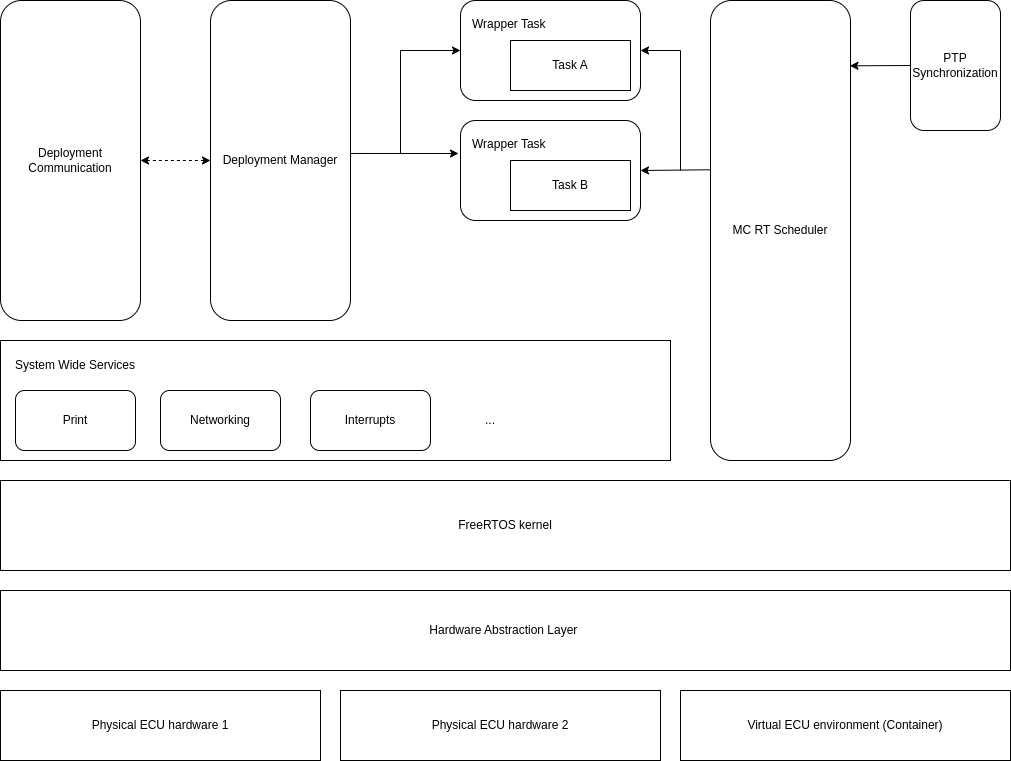
\includegraphics[width=\textwidth]{figures/os_arch_extended.png}}
\end{center}


\begin{itemize}
	\item Extended Scheduler (Mixed Criticality and Real-Time Capable) - Based on ESFREE extension
	\item Task Deployment Communication Handler: Responsible for receiving instructions and task executables from a master node, as well as sending back messages about the status of the running system	
	\item Task Deployment Manager:  as well as triggering the dynamic control of the tasks (creation/destruction and start/stop/pause), as well as sending/receiving the checkpoint data. This includes the process of loading the ELF applications onto the system's memory.
	\item Wrapper Task: The user tasks, sent by the master node, shall be encapsulated in ELF files containing the machine code for them to run on top of the OS. However, as the core behavior of FreeRTOS does not contemplate loading of external applications, a wrapper task will allow for this feature. This wrapper task will handle some common functionalities for the user real-time tasks, such as: real-time constraint keeping, management of application stack and checkpoints, and passing handles for system functions to the applications
	\item System function services: these are services that are exposed to the user applications as "system functions". Since the microkernel architecture makes it tricky to handle some services globally by not offering shared libraries, some common functionalities (e.g. network communication or console prints) are offered by system services and passed via the wrapper task to the applications 
\end{itemize}

\section{Mixed Criticality Scheduler}

The first step in achieving mixed criticality and respecting real-time behavior for the system applications is a scheduler that can achieve both goals. For this purpose, an extension of ESFREE (add reference), a project that implements a few dynamic and static real-time scheduling policies, including Earliest Deadline First (EDF), which for single core is ideally optimal (add references). This project is used as a base as the off-the-shelf FreeRTOS code only offers a priority-based scheduler, without any priority-assignment policies. In this work, the EDF policy is extended to cope with different levels of criticality by implementing the EDF with virtual deadlines for MC, as proposed in (add ref.).  

\section{Cross-Platform Task Loading}

To achieve the goal of executing the same application files on both physical and virtual ECU devices, the system integrates an ELF loader. This ELF loader, mostly implemented in the scope of the master's thesis of Yinbo Zhou (cite), enables the execution of multiple tasks, packed in the form of pre-compiled ELF files and with an additional data file. This approach tackles both challenges of allowing the dynamic loading of tasks and of stateful migration to the extent desired. In order for applications to be compatible with the task loader, they need to fulfill some requirements when compiled.  